\documentclass[12pt,a4paper,ngerman,twoside]{scrbook}

\usepackage{babel}
\usepackage[utf8]{inputenc}
\usepackage{lmodern} % besserer schriftsatz
\usepackage{graphicx}
\usepackage{siunitx}	% \[\SI{100}{\electronvolt}\] %BLOCK % \SI{100}{\electronvolt} %Fliesstext
\sisetup{
  locale = DE ,
  per-mode = symbol,
  output-decimal-marker={.}
}
\usepackage{float}
\usepackage[labelfont={bf,sf},font={small,it},% Optionen für Abbildungstexte
  labelsep=space]{caption}
\usepackage{amsmath,amssymb} %align for math
\usepackage{hyperref,cleveref}
\usepackage{url}
\usepackage{todonotes}
\urlstyle{same}
\usepackage{pdfpages}
\setlength\parindent{0pt}

\newcommand{\newlines}{\newline\newline}

\begin{document}
\begin{titlepage}
	\centering
	\includegraphics[width=0.3\textwidth]{illustrations/tu_logo.png}\par\vspace{1cm}
	{\scshape\LARGE Technische Universit\"at Berlin \par}
	\vspace{1cm}
	{\scshape\Large Bachelorarbeit\par}
	\vspace{1.5cm}
	{\Large\bfseries Validierung einer Simulation von Selbstabsorptionseffekten bei Fluoreszenz-Nanoskopie\par}
	\vspace{2cm}
	{\Large\itshape Conrad Dollinger\par}
	\vfill
	
	Erstgutachterin: Prof. Dr. Birgit  \textsc{Kanngie\ss er}\par
	Zweitgutachter: Dr. Burkhard \textsc{Beckhoff}\par
	\vspace{0.5cm}
	Betreuer: Dr. Lars \textsc{Lühl}\par
	\vfill
	Fakultät II - Mathematik und Naturwissenschaften\par
	Institut für Optik und Atomare Physik\par 
	AG Analytische Röntgenphysik \par
\vspace{0.5cm}
	{\large 10. Juli 2018\par}
\end{titlepage}
%Eine leere Seite einfügen 
\newpage 
\thispagestyle{empty} %plain, empty[keine Kopf/Fusszeile], headings[Fusszeile wird zur Kopfzeile]
\addtocounter{page}{-1}
\quad
%einfügen Ende

\newpage
\thispagestyle{empty} %plain, empty, headings
\includepdf[pages={1}]{erklaerung.pdf}
\addtocounter{page}{-1}

%Eine leere Seite einfügen 
\newpage 
\thispagestyle{empty} %plain, empty[keine Kopf/Fusszeile], headings[Fusszeile wird zur Kopfzeile]
\addtocounter{page}{-1}
\quad
%einfügen Ende


\newpage
\pagenumbering{Roman} % set the numbering style to Roman:uppercase roman numerals
\tableofcontents

\newpage
\thispagestyle{empty}
\pagenumbering{arabic} % set the numbering style to arabic numbers
\setcounter{page}{0} % Set the page counter to 1
\section*{Einleitung}
Röntgenmikroskopie ist ein Bildgebungsverfahren, welches ein Auflösungsvermögen zwischen einem Lichtmikroskop und SEM (\textit{scanning electron microscope}) besitzt. Dabei kann das Transmissionssignal mittels STXM (\textit{scanning transmission X-ray microscopy}) detektiert werden. Außerdem ist es möglich den Aufbau um einen optionalen Fluoreszenzdetektor zu erweitern, wie im Fall des AnImaX-Projekts (\textit{Analytical Imaging with X-Rays}) der AG Kanngießer (TU Berlin). Das Projekt beschäftigt sich im Themengebiet der Röntgenfluoreszenz an einem Aufbau, welcher gleichzeitige Detektion von Fluoreszenzsignalen, sowie die dazugehörigen Transmissionssignalen erlaubt. Dafür wurde eigens ein QUAD Silizium Drift Detektor (SDD) von \textit{Bruker Nano} angefertigt, welcher im AnImaX Röntgenmikroskop verbaut ist. Der Detektor ermöglicht die Aufnahme eines großen Raumwinkels ($>\SI{1}{\steradian}$), daher ist er beispielsweise für biologische Proben, welche nur ein schwaches Fluoreszenzsignal emittieren, geeignet. \newline
Durch den großen Raumwinkel bedingt sind herkömmliche Quantifizierungsansätze für diesen Detektor nicht mehr gültig. Die Fluoreszenzstrahlung kann nicht mehr als parallel angenommen werden, da sie verschiedene Pfade durch die Probe nimmt. Je nach Aufbau der Probe variieren daher sowohl die Weglänge durch die Probe, als auch die Absorptionskoeffizienten aufgrund wechselnder chemischer Kompositionen. \newline
Als Teil der Arbeit \textit{Simulation of Solid Angle Effects in the Detection of X-ray Fluorescence upon Investigation of Inhomogeneous Samples} von Hanna Dierks ist dadurch das Simulationsprogramm QUADaps entstanden, welches diese Effekte aufgrund einer virtuellen Beschreibung des QUAD Detektors simuliert und Grundsteine für eine Quantifizierung in der Röntgenfluoreszenz unter großen Raumwinkeln legen soll. \newline
In dieser Arbeit soll nun an erste Ergebnisse angeknüpft werden. Das Hauptaugenmerk liegt auf dem Entwurf von Proben, welche in den nachfolgenden Kapiteln logisch aufgebaut werden. Diese sollen simuliert und im Anschluss an diese Arbeit experimentell untersucht werden. Der Vergleich von simulierten und experimentell ermittelten Daten soll zur Validierung des Simulationsprogramms QUADaps beitragen.



\chapter{Theoretischer Hintergrund}	%Arbeitstitel
\section{Röntgenstrahlung}
Die Entdeckung der Röntgenstrahlung gelang Wilhelm Conrad Röntgen 1895 durch Beobachtungen von Fluoreszenzeffekten an Bariumplatincyanür in der Nähe einer Elektronenröhre (org.: \textit{Hittorf'sche Vacuumröhre}). Diese war eigentlich mit einem schwarzen Karton ummantelt und die im inneren entstehende Strahlung sollte dadurch nach bisherigem Kenntnisstand abgeschirmt sein. Damals vermutete Röntgen, dass die von ihm entdeckten X-Strahlen longitudinale Schwingungen aus dem Äther seien \cite[Absätze~1,2,17]{wcrpaper}. Heute wissen wir, dass es sich bei Röntgenstrahlen um transversale, elektromagnetische Strahlung in einem Energiebereich von etwa \SI{15}{\electronvolt} bis zu etwa \SI{1.2}{\mega\electronvolt} handelt, wobei die Grenzen zwischen UV- und Röntgenstrahlung im unteren Energiebereich bei etwa \SI{10}{\electronvolt} bis \SI{500}{\electronvolt}  und zwischen Röntgen- und Gammastrahlung im oberen Energiebereich um ca. \SI{500}{\kilo\electronvolt} nicht fest definiert sind.\newline

\begin{figure}[H] %h:Grafik an dieser Stelle einbinden. Falls das nicht geht: %t:oben auf der Seite. Wenn dies auch nicht möglich ist: %b:am Fuß der Seite oder %p:auf der nächsten Seite %! is specified, then ignore the restrictions of placing floating objects %H (float package) forces position
  \centering
     \includegraphics[width=0.9\textwidth]{illustrations/spectrumEMradiation.png}
  \caption[Spektrum EM-Strahlung]{Darstellung des Spektrums elektromagnetischer Strahlung von infrarotem(IR), über sichtbares(VIS) und ultraviolettem(UV) Licht bis zu Röntgenstrahlung. Außerdem sind die Abstufungen des UV Lichts in vacuum(VUV) und extrem(EUV), weiche und harte Röntgenstrahlung und das Wasserfenster dargestellt. \cite[S.~34]{bbbook}}
  \label{fig:spectrumEMradiation}
\end{figure}

\noindent Die Erzeugung von Röntgenstrahlen kann auf 2 Arten geschehen: Einerseits entsteht durch das Ablenken von Elektronen die sog. "Bremsstrahlung"\,\,(\cref{fig:spectrumXray}) welche zu einem kontinuierlichen Spektrum führt und die Röntgen wohl ursprünglich indirekt beobachtet hat. Andererseits liefern Schalenübergänge von Elektronen ein sog. charakteristisches Röntgenspektrum welches sich eindeutig Elementen zuordnen lässt. Im Hintergrund dieser Arbeit ist das Verständnis beider Arten von Nöten. Wird ein Elektron in einem elektrischen Feld auf die Energie $E_{kin} = e \cdot U$ beschleunigt und daraufhin durch Magnetfelder auf einer Kreisbahn gehalten, wie beispielsweise in einem Beschleuniger oder Synchrotron \cite[S.~33]{bbbook}, so kann es in einem Undulator so abgelenkt werden, dass Bremsstrahlung ensteht, welche ein absorbierendes Atom zur Fluoreszenz seiner charakteristischen Linien anregen kann.\newline

\begin{figure}[H] %h:Grafik an dieser Stelle einbinden. Falls das nicht geht: %t:oben auf der Seite. Wenn dies auch nicht möglich ist: %b:am Fuß der Seite oder %p:auf der nächsten Seite %! is specified, then ignore the restrictions of placing floating objects %H (float package) forces position
  \centering
     \includegraphics[width=0.9\textwidth]{illustrations/XrtSpectrum_edit.png}
  \caption[Röntgenspektrum charakteristisch und kontinuierlich]{Abgebildet ist ein typisches Röntgenspektrum, bestehend einerseits aus den charakteristischen Peaks der Schalenübergänge und andererseits aus einem kontinuierlichen Bremsspektrum. Das Abflachen im niederenergetischen Bereich wird durch Wechselwirkung der Photonen mit Materie bedingt, im Vakuum gibt es daher kein Abflachen (gestrichelt) \cite[bearbeitet]{spectrum}.}
  \label{fig:spectrumXray}
\end{figure}


\section{Röntgenfluoreszenz}
Wird ein Atom durch die Absorption eines Röntgenphotons ionisiert, sodass ein Elektron aus einer inneren Schale mit dem Energieniveau $E_k$ das Atom verlässt, so kann ein beliebiges Elektron des Atoms mit der Energie $E_i > E_k$ in den freien Zustand zurückfallen, insofern dieser Übergang erlaubt ist. Dabei wird ein Fluoreszenzphoton gemäß $h \cdot \nu = E_i - E_k$ frei \cite[S.~261]{dem3}.

\begin{figure}[H] 
  \centering
     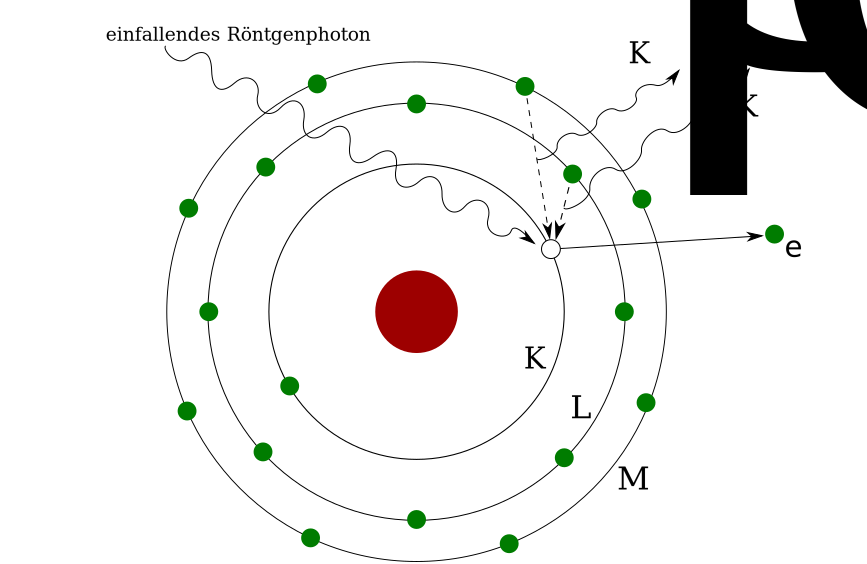
\includegraphics[width=0.65\textwidth]{illustrations/fluorescence.png}
  \caption[Skizze Fluoreszenz]{Die Erzeugung von Fluoreszenzphotonen durch vorherige Anregung mit einem Röntgenphoton ist hier abgebildet. Zur Veranschaulichung sind die Energieniveaus im Bohr'schen Atommodell gezeichnet \cite[S.~25, bearbeitet]{hanna}.}
  \label{fig:fluoreszenz}
\end{figure}

\noindent Wie in \cref{fig:fluoreszenz} dargestellt sind die Fluoreszenzlinien nach den Übergängen benannt. So entsteht beispielsweise ein Photon der $K_{\beta}$-Linie beim Übergang eines Elektrons von der $M$-Schale in die $K$-Schale eines Atoms unter Emission eines Photons der Energie $E_M - E_K$. Die möglichen Energieniveaus der Elektronen eines Atoms sind durch seine Quantenzahlen bestimmt. Diese sind für unterschiedliche Elemente nicht gleich. Daher sind auch die möglichen Energieniveaus der Elektronen nicht gleich. Demzufolge lassen sich die durch Fluoreszenz ausgelösten Elektronen über ihre Energie einem Element zuordnen. Man spricht bei diesem Effekt von charakteristischer Röntgenstrahlung.

\section{Silizium Drift Detektoren}

Die Detektion von ionisierender Strahlung durch Silizum Drift Detektoren (SDD) ist seit der Einführung 1983 von E. Gatti und P. Rehak möglich. SDDs zeichnen sich besonders durch eine sehr hohe Energieauflösung und eine kurze Totzeit aus. Letzteres ist die Grundlage moderner Bildgebungsverfahren bei Röntgenspektroskopie, da diese auf relativ hohe Photonenflussraten angewiesen ist.   
SDDs bieten eine hohe Flexibilität, da sie bei relativ hohen Temperaturen (um \SI{250}{\kelvin}) und mit größeren aktiven Flächen betreibbar sind als Si/Li-Detektoren. Außerdem profitieren sie von einem sehr guten Verhältnis von Signal zu elektrischem Rauschen. Heutzutage haben SDDs die meisten Si/Li-Detektoren vollständig abgelöst.\newline

Das Wirkungsprinzip der SDDs lässt sich ausgehend von Verarmungszonen, welche bei herkömmlichen bipolaren Transistoren bereits bekannt sind, gut beschreiben. Beim Betrachten des Querschnitts eines SDD strecken sich an Ober- und Unterseite des Detektors die p-Elektroden über etwa $\frac{2}{3}$ der Detektorfläche, während sich die kleine n-Elektrode etwas räumlich getrennt befindet. Durch diese Struktur bildet sich seitlich eine Verarmungszone aus wie in \cref{fig:sdd_concept} dargestellt. 

\begin{figure}[H] 
  \centering
     \includegraphics[width=0.85\textwidth]{illustrations/sdd_concept.png}
  \caption[Prinzip eines SDD]{Schematisch abgebildet ist das Wirkungsprinzip eines Silizum Drift Detektors. Von den gegenüberliegenden p-Elektroden bildet sich eine Vararmungszone seitwärts zur n-Elektrode hin aus \cite[S.~223, bearbeitet]{bbbook}.}
  \label{fig:sdd_concept}
\end{figure}

Außerdem wird durch konzentrische Ringe auf der Rückseite des SDD ein weiteres elektrisches Feld parallel zur Detektoroberfläche so angelegt, dass die durch die ionisierende Strahlung ausgelösten Elektronen seitlich zur n-Anode beschleunigt werden. Veranschaulicht kann man sich \cref{fig:sdd_concept} so vorstellen, dass die p-Elektroden senkrecht zur Oberfläche in kleinere Elemente zerlegt sind und zwischen diesen eine kleine Potentialdifferenz für die Beschleunigung, den Drift, der Elektronen sorgt. Später werden die Elektronenladungen durch einen Feldeffekttransistor in eine Spannung proportional zu den ausgelösten Elektronen und damit zur Photonenenergie der eintreffenden Röntgenstrahlung umgewandelt, welche nachfolgend von einem Multi-Channel-Analyser ausgewertet werden kann.




\section{Detektor- und Streuungseffekte}
Nachdem im vorangestellten Abschnitt auf das Wirkungsprinzip eines SDD eingegangen wurde, soll in diesem Abschnitt auf beobachtbare physikalische Effekte eingegangen werden, welche als Messartefakte in den detektierten Daten hinterbleiben. Diese können beispielsweise durch die Art des Detektors, allgemein aber auch durch diverse Streuprozesse wie elastische (Rayleigh) oder inelastische Streuung (Compton) bedingt sein. Ignorieren dieser Effekte würde zwangsweise zu falsch interpretierten Daten führen, wie am folgenden Beispiel ersichtlich:\newlines
Erreichen 2 Photonen einer monochromatischen Quelle die aktive Detektorfläche zwischen zwei Ausleseperioden, so sind die durch die Photonen ausgelösten Ladungsträger\-wolken für die Ausleseelektronik voneinander ununterscheidbar. Dadurch wird die voll\-ständige Ladung einem Photon mit der doppelten Photonenenergie zugeordnet, Pile-Up-Effekt genannt. Dieser Effekt tritt signifikant nur bei verhältnismäßig hohen Zählraten auf. Moderne SDD Sofware bietet bereits die Möglichkeit, die Ausleserate an die Zählrate anzupassen. Außerdem geschieht das Auslesen der Ladungsträgerwolken durch 2 Kanäle: 1 Kanal mit sehr kurzer Auslesezeit, dafür schlechter Energieauflösung und ein Kanal mit langsamer Auslesezeit und besserer Energieauflösung. Wird im schnellen Kanal nur 1 Count registriert, so wird die im langsamen Kanal detektierte Energie ausgewertet. Werden im 1. Kanal mehrere Counts registiert, so wird das Ergebnis aus Kanal 2 verworfen und die Counts tragen zur Berechnung der Totzeit mit bei. Treffen jedoch 2 Photonen in so kurzem Abstand voneinander ein, dass der 1. Kanal diese als 1 Count zusammenaddiert, spricht man von einem Pile-Up-Effekt. Glücklicherweise lassen sich bei Röntgenfluoreszenzspektroskopie die falsch zugeordneten Signale auch manuell sehr leicht identifizieren denn die Energien entsprechen einer Summe aus diskreten Röntgenlinien.\newlines
Ein weiterer, regelmäßig auftretender Effekt ist die unvollständige Detektion der Ladungsträgerwolken durch Verlust von Elektron-Loch-Paaren auf dem Weg zur Ausleseelektronik. Dies liegt vor Allem an im Bereich der Oberfläche ausgelösten Elektronen. Die Eindringtiefe niederenergetischer Photonen in die Detektorfläche ist sehr gering. Demzufolge wird ein größerer Anteil der ausgelösten Ladungsträger nahe an der Oberfläche ausgelöst, wo sie entweder Rekombinieren oder ihre Ladung an die Elektrode abgeben können. Dieser Effekt wird durch flache Einfallswinkel verstärkt, unter welchen die Photonen einen längeren Weg durch die oberste Schicht der aktiven Fläche passieren müssen.\newlines
Wird ein Atom durch Strahlung ionisiert, so wird ein Anteil entsprechend $E_{kin} = h\nu - E_{bind}$ der Photonenenergie dem aus einer inneren Schale ausgelösten Elektron als kinetische Energie mitgegeben. Dieses löst durch Stoßprozesse eine Ladungsträgerwolke aus. Ein freies Elektron oder ein Elektron einer äußeren Schale wird den freigewordenen Platz in der inneren Schale einnehmen. Dabei kann es die freiwerdende Energie entweder als Auger-Elektron auf ein andere Elektron übertragen oder diese abstrahlen. Das Auger-Elektron wandelt seine Energie auch in eine Ladungsträgerwolke um, das Photon kann jedoch auch aus der Oberfläche austreten. Dadurch ist die detektierte Energie genau um die Energie des emittierten Photons niedriger. Es entstehen leicht zu identifizierende Peaks im Abstand der Photonenenergie des Si-Photons. Zur Korrektur ist es ausreichend die beiden Peaks mit und ohne Escape-Peak zu summieren.\newlines
Der Vollständigkeit halber werden noch Bragg-Peaks, welche mit Einfalls- und Ausfallswinkel in eine spezifische kristalline Struktur korrellieren, genannt. Sie werden von der Bragg-Bedingung beschrieben und treten vorherrschend bei höheren Photonenenergien auf. In den in dieser Arbeit zu untersuchenden Proben sind Bragg-Peaks jedoch nicht in signifikantem Umfang zu erwarten, da biologische Proben meist keine kristalline Struktur aufweisen.

\chapter{AnImaX-Projekt und QUADaps-Software}	%Arbeitstitel
\section{AnImaX Projekt}
Die Entwicklung des AnImax-Projekts entspringt als ein Teil des FlexIX-Projekts des Bundesministerium für Bildung und Forschung. Das Kooperationsprojekt zwischen der TU Berlin und der Hochschule Koblenz wurde ursprünglich als Messstation für die P04 Beamline bei Petra III (DESY Hamburg) entworfen, kann jedoch auch an anderen Synchrotrons (z.B. BESSY II, HZB Berlin) mit einer Energiespanne von \SI{200}{\electronvolt}-\SI{3000}{\electronvolt} genutzt werden. Es handelt sich um einen experimentellen Aufbau mit STXM im full-field-Modus oder STXM mit optionaler Detektion des Fluoreszenzsignals.
\subsection{Experimenteller Aufbau}
Der optische Aufbau (\cref{fig:animaxsetup}) befindet sich in einer Messkammer im Hochvakuum bei etwa \SI{e-6}{\milli\bar}. Davor ist eine weitere Messkammer im Hochvakuum (\SI{5e-7}{\milli\bar}) direkt an die Beamline angeschlossen. Sie dient als differentielle Pumpstrecke für das Ultrahochvakuum der Beamline (\SI{e-9}{\milli\bar}). Aus dem von der Beamline kommenden Synchrotronstrahl wird eine Wellenlänge selektiert. Der Strahl trifft auf eine Fresnelsche Zonenplatte mit einer Brennweite von \SI{7}{\milli\meter} (bei \SI{700}{\electronvolt}). Die äußere Zonenweite ist \SI{45}{\nano\meter}, der Außendurchmesser beträgt \SI{333}{\micro\meter}. Die Mittenstop hat einen Durchmesser von \SI{160}{\micro\meter} und filtert gemeinsam mit der OSA (OSA = \textit{order sorting aperture}) zusammen alles bis auf die 1. Ordnung des von der Zonenplatte gebeugten Lichts aus. Die OSA ist ein Pinhole mit \SI{150}{\micro\meter} Durchmesser und befindet sich mit der Zonenplatte auf einem gemeinsamen Frame, über Piezekristalle lässt sich der Abstand zwischen beiden jedoch justieren. Außerdem ist sie an einem Röhrchen fixiert, welches sich in die zentrale Öffnung des QUAD-Detektors bewegen lässt. Der Synchrotronstrahl wird also an der Zonenplatte fokussiert und passiert die OSA und das zentrierte Loch des Detektors bevor er auf die Probe trifft. Daraufhin wird ein Teil der Strahlung in Fluoreszenz umgewandelt und vom SDD registriert. Die durch die Probe transmittierte Intensität kann durch eine schnellauslesende CCD außerhalb der Messkammer detektiert werden. Da CCDs für Röntgenstrahlung die benötigten Zählraten nicht leisten können, wurde auf eine CCD, welche sensitiv für sichtbares Licht ist, zurückgegriffen. Daher ist hinter der Probe noch ein Phosphorschirm angebracht, welcher sichtbares Licht (grün) emittiert. Dieses wird durch eine Linse gesammelt und über ein Bleifenster aus der Vakuumkammer ausgekoppelt, dann durch die CCD detektiert.

\begin{figure}[H] %h:Grafik an dieser Stelle einbinden. Falls das nicht geht: %t:oben auf der Seite. Wenn dies auch nicht möglich ist: %b:am Fuß der Seite oder %p:auf der nächsten Seite %! is specified, then ignore the restrictions of placing floating objects %H (float package) forces position
  \centering
     \includegraphics[width=0.9\textwidth]{illustrations/animax-gruppe_hanna.png}
  \caption[Skizze optischer Aufbau]{Der optische Aufbau im AnImaX-Projekt. Die von der Synchrotronquelle eintreffene Strahlung wird zunächst an der Zonenplatte fokussiert, höhere Ordnungen werden an der OSA aussortiert. Der Strahl passiert den QUAD-Detektor zentral und trifft auf die Probe, welche zur Fluoreszenz angeregt wird. Hinter der Probe wandelt ein Phosphorschirm das transmittierte Licht in eine für die CCD sichtbare Wellenlänge um. Das Licht wird mit Hilfe einer Linse parallelisiert und von der CCD detektiert wird \cite[S.~40]{hanna}.}
  \label{fig:animaxsetup}
\end{figure}
Über Piezokristalle lässt sich der Probenhalter bewegen. An diesem befindet sich Platz für 5 Proben, sodass ein Probentausch ohne Brechen des Vakuums möglich ist. Die Piezokristalle lassen sich x- und y-Richtung enkodiert mit einer Genauigkeit von etwa \SI{0.1}{\nano\meter} und einer Reichweite von \SI{100}{\micro\meter} fahren. Dies ermöglicht eine hohe Auflösung bei großer abgerasterter Fläche. Der Scanner Frame und damit auch die Probe können mit Hilfe einer Computersoftware gesteuert werden. Dazu sind die Piezokristalle an einen Controller und dieser an einen PC angeschlossen. Zwei Scan-Modi stehen zur Datenakquise zur Verfügung: der step-by-step-Modus und der on-the-fly-Modus, welcher kontinuierlich Daten akquiriert. Letzterer ermöglicht deutlich verkürzte Messzeiten, eine Messung mit 10000px je \SI{200}{\milli\second} Aufnahmezeit benötigt beispielsweise nur etwa eine halbe Stunde.\newlines

\section{Beschreibung der Detektorgeometrie}
Beim einzigartigen QUAD-Detektor (\cref{fig:aufbau_foto} B) von \textit{Bruker Nano} handelt es sich um einen 4-Kanal SDD. Die vier baugleichen, voneinander unabhängigen, nierenförmigen SDD-Zellen sind symmetrisch so um das Pinhole angeordnet, dass sie einer Kreisscheibe möglichst nahe kommen, ohne das Pinhole zu verdecken. Zum Schutz vor Fotoelektronen ist ein \SI{0.5}{\micro\meter} dickes Mylar-Fenster  angebracht. Durch dieses können Elektronen bis maximal etwa \SI{3}{\kilo\electronvolt} abgeschirmt werden. Durch das Pinhole wird der von der Zonenplatte fokussierte Strahl auf die Probe gebracht. Dementsprechend zeigen die Detektorflächen in Strahlrichtung und sitzen möglichst parallel gegenüber zur Probenoberfläche. Der Chip des QUAD-Detektor ist quadratisch und besitzt eine Außenkantenlänge von \SI{14}{\milli\meter} obwohl die Breite der aktive Fläche kleiner ist. Die Gesamtfläche einer nierenförmigen Zelle beträgt \SI{11.2}{\square\milli\meter}. Vom äußersten Rand der Nierenzellen ($r_a=$ \SI{5.1}{\milli\meter}) ausgehend, decken die 4 Zellen gemeinsam 54.8\% der Kreisfläche mit gleichem Radius ab.
\begin{figure}[H]
  \centering
     \includegraphics[width=0.9\textwidth]{illustrations/aufbau-foto_hanna.png}
  \caption[Foto der Optiken und des QUAD-Detektor]{Foto des optischen Aufbaus um den QUAD-Detektor. A) zeigt die Zonenplatte und OSA auf einem röhrenförmigen Support. B) links: QUAD-Detektor in Seitansicht; rechts: in Draufsicht. C) zeigt eine Probe auf der Scanner-Stage, D) Phosphorschirm \cite[S.~41]{hanna}.}
  \label{fig:aufbau_foto}
\end{figure}
Soll der detektierte Raumwinkel maximiert werden, gilt es zu beachten, dass durch den Metallrahmen, welcher den Detektor umgibt Teile der Detektorfläche abgeschirmt werden. Außerdem fügt der Rahmen ein z-Offset $d_{off} = d_{in} + d_{R}$ zum realen Abstand Probenoberfläche zu SDD hinzu. Eine schematische Skizze der Geometrie zwischen Probe und Detektor ist nachfolgend illustriert (\cref{fig:quaddetektor}).
\begin{figure}[H]
  \centering
     \includegraphics[width=0.9\textwidth]{illustrations/winkel.png}
  \caption[Detektorgeometrie im Detail]{Detektorgeometrie im Detail. Im Lot der Probenoberfläche (beige) trifft die Synchrotronstrahlung ein. Davon ausgehend sind die Winkel $\alpha$ und $\beta$ aufgetragen, die den inneren, respektive äußeren Detektionsradius begrenzen. Der Detektor (blau) wird radial durch $r_{max}$ begrenzt. Das Mylar-Fenster (cyan) ist in den Metallrahmen (grau) eingebettet welcher im Abstand $d_{in}$ zum Chip befestigt ist. Der Winkel $\beta$ wird durch eine Kante im Rahmen bei ($r_{Ri},\,d+d_{R}$) begrenzt. Für $\alpha$ müssen die Kanten ($r_{La},\,d+d_{f}$) und ($r_{Li},\,d+d_{L}$) in Betracht gezogen werden. In Millimeter: $r_{Ri}=5.1$, $r_{Li}=2.5$, $r_{La}=1.9$, $r_{max}=7.0$, $d_{in}=0.4$, $d_{R}=1.15$, $d_{L}=0.9$, $d_{f}=0.1$.}
  \label{fig:quaddetektor}
\end{figure}
Zunächst soll berechnet werden für welche Proben-Detektor-Abstände $d$ die Rahmenkante bei ($r_{La},\,d+d_{f}$) und ansonsten die bei ($r_{Li},\,d+d_{L}$) den Innenwinkel $\alpha$ begrenzen. Dazu wird das Koordinatenzentrum in die eintreffende Strahlung auf der Probenoberfläche gelegt. Es lässt sich folgende Steigungsgleichung aufstellen:
\begin{equation}
m = \frac{\Delta y}{\Delta x} = \frac{y_2-y_1}{x_2-x_1} = \frac{(d+d_{L})-(d+d_{f})}{r_{Li}-r_{La}} = \frac{0.9-0.1}{2.5-1.9} = \frac{0.8}{0.6} = \frac{4}{3} .
\end{equation}
Somit ergibt sich der kritische Abstand $d_{crit}$ unter dem die äußere Kante den minimalen Einfallswinkel limitiert zu:
\begin{equation}
d_{crit} + d_f = m \cdot r_{La} \Leftrightarrow (1.9 \cdot \frac{4}{3})-0.1 = d_{crit} = \SI{2.43}{\milli\meter} .
\end{equation}
Das heißt, dass $\alpha$ bei einem Abstand unter $d_{crit} =$ \SI{2.43}{\milli\meter} von ($r_{La},\,d+d_{f}$), überhalb von ($r_{Li},\,d+d_{L}$) begrenzt wird. Daraus ergeben sich folgende Beziehungen für die Winkel $\alpha$ und $\beta$:
\begin{equation} \label{alpha1}
\tan(\alpha) = \frac{r_{La}}{d+d_f} \quad,\quad d \leq \SI{2.43}{\milli\meter}
\end{equation}
\begin{equation} \label{alpha2}
\tan(\alpha) = \frac{r_{Li}}{d+d_L} \quad,\quad d > \SI{2.43}{\milli\meter}
\end{equation}
\begin{equation} \label{beta}
\tan(\beta) = \frac{r_{Ri}}{d+d_R}.
\end{equation}
Im nächsten Schritt soll der detektierte Raumwinkel $\Omega$ bestimmt werden. Der kanonische Raumwinkel (Kreissegment einer Kugeloberfläche) berechnet sich mit dem Öffnungswinkel eines Kegel $\omega$ nach: 
\begin{equation}
\Omega = 2 \pi (1-\cos(\frac{\omega}{2})).
\end{equation}
Der detektierte Raumwinkel ergibt sich also aus der Differenz des doppelten äußeren und inneren Raumwinkels:
\begin{equation} \label{raumwinkel}
\Omega = \Omega_{2\beta}-\Omega_{2\alpha} = 2 \pi (1-\cos(\beta)) - 2 \pi (1-\cos(\alpha)) = 2 \pi (\cos(\alpha) - \cos(\beta)).
\end{equation} % maximize y = 2pi(cos(arctan(2.5/(x+0.9)))-cos(arctan(5.1/(x+1.15))))	% maximize y = 2pi(cos(arctan(1.9/(x+0.1)))-cos(arctan(5.1/(x+1.15))))
Maximieren von \cref{raumwinkel} mit \cref{alpha1} und \cref{beta} liefert ein Maximum $\Omega_{max} = \SI{1.41}{\steradian}$ am Rand bei $d = \SI{2.43}{\milli\meter}$. Die analoge Rechnung mit \cref{alpha2} und \cref{beta} liefert ein lokales Maximum außerhalb des Definitionsbereichs ($<$\SI{2.43}{\milli\meter}).\newlines
Es ergeben sich dadurch im optimalen Probe-Detektor-Abstand ein innerer Öffnungswinkel $\alpha = \SI{36.9}{\degree}$ und ein äußerer Öffnungswinkel $\beta = \SI{54.9}{\degree}$. \newline Das gefundene Ergebnis liegt außerdem innerhalb der Begrenzung der aktiven Zone $r_{max}=\SI{7}{\milli\meter}$: $r = (d+d_R+d_{in})\cdot \tan(\SI{54.9}{\degree}) = \SI{5.64}{\milli\meter}$. \newline
Zudem wird der detektierte Raumwinkel noch durch den nierenförmigen Rahmen gesenkt. Zur Approximation wird die durch die Nieren abgedeckte Fläche im Verhältnis zur Ringscheibe mit gleichen Radien gesetzt, dies entspricht etwa 72\%. Der real detektierte Raumwinkel ergibt sich damit zu $\Omega_{real} = \Omega_{max} \cdot 0.72 = \SI{1.02}{\steradian}$.
\subsection{Absorptionseffekte durch großen Raumwinkel}
Ein großer detektierter Raumwinkel ($>\SI{1}{\steradian}$) ist gleichbedeutend mit einer großen Variation an Beobachtungswinkeln. Dies widerspricht den klassischen Quantifizierungsansätzen für Röntgenfluoreszenzanalyse basierend auf der Sherman-Gleichung, welche mit einer Näherung für kleine detektierte Raumwinkel arbeiten.\newline
Obwohl bereits explizit für große Winkel diverse Ansätze für die Sherman-Gleichung überprüft wurden (Bonizoni et al., 2006; Chang and Wittry, 1994; Malzer and Kanngießer, 2003; Mantler and Kawahara, 2004; Pavlinsky and Kitov, 1979), existiert dafür bisher keine vollständig analytische Integration in die Sherman-Gleichung. Jedoch gibt es für homogene Proben den \textit{equivalent angle}-Ansatz (Malzer und Kanngießer, 2003) welcher zur Quantifizierung dieser Ergebnisse genutzt werden kann. Im Fall von inhomogenen Proben muss jedoch noch ein verlässlicher Quantifizierungsansatz gefunden werden \cite[Abs.~1.2.2]{lars}.
\section{QUADaps Software}
Um die besondere Detektor-, und diverse Probengeometrien zu simulieren wurde die Simulationssoftware \textbf{QUADaps} nach den 4 Detektorzellen (\textbf{QUAD}) sowie \glqq\textbf{a}bsorption \textbf{p}ath \textbf{s}imulations\grqq entwickelt. Dabei basieren die Berechnungen und Simulationen auf dem Softwarepaket \textit{xrfLibrary}, welches von der AG Kanngießer (TU Berlin) entwickelt wurde. Als Datenbanksatz wird die Elam Datenbank aus dem Paket \textit{xrlfupa} genutzt. Dieses enthält die fundamentalen Röntgenstrahlungsparameter und einen großen Datensatz an optischen Parametern. Mithilfe der \textit{xrfLibrary} werden dann Quellen (\textit{source()}), Proben (\textit{specimen()}), Filter (\textit{filter()}) und Detektoren (\textit{detector()}) definiert. Um eine Fluoreszenzsimulation zu erstellen wird zunächst eine monochromatische Quelle (\textit{monoSource()}) erstellt und ihr die gewünschte Photonenenergie $E$ und Intensität $I_{0}$ übergeben. \newline
Daraufhin muss die zu untersuchende Struktur erstellt werden. Dazu dient ein xy-Raster (\textit{layoutXY}) (\cref{fig:xyc_layout}) mit beliebig, wahlweise unterschiedlich großen Rasterpunkten, welches die 2-dimensionalen Abmessungen der Struktur in Draufsicht widerspiegelt. Über dieses Raster wird ein gleich großes Raster gelegt (\textit{layoutC}), welches an jedem Punkt die Informationen über das lokale Probendesign enthält. Genauer werden in \textit{layoutC} Probenobjekte (\textit{specimen()}) nebeneinandergereiht. 

\begin{figure}[H]
  \centering
     \includegraphics[width=0.9\textwidth]{illustrations/xyc_layout.png}
  \caption[2D-Visualisierung von layoutXY]{Eine 2D-Visualisierung von \textit{layoutXY}. Die Größe der einzelnen Gitterzellen wird bestimmt durch die Breite der jeweiligen $x_i$ und $y_i$. Es können beliebig viele Zellen erstellt und unabhängig groß voneinander gewählt werden. \textit{layoutC} ordnet jeder Zelle ein \textit{specimen()}-Objekt (hier 0,1,2) zu welches Informationen über die gestapelten Schichten enthält.}
  \label{fig:xyc_layout}
\end{figure}



Jedes Probenobjekt besteht aus einer oder mehreren Schichten (\textit{layers}) beliebiger Höhe, sodass hier das Höhenprofil, die z-Komponente, der zu untersuchenden Struktur abgebildet wird. Eine Schicht hingegen ist ein Quader einer homogenen Komposition chemischer Elemente (\textit{compound}) sowie der dazugehörigen Dichte. Veranschaulicht ist dies in \cref{fig:specimen}. Folglich zeigt sich, dass das Simulieren von Inhomogenitäten sehr aufwändig ist, da diese einzeln in die homogenen Strukturen eingearbeitet werden müssen. Außerdem sollte die Ausrichtung des Objekts auf den Detektorachsen liegen, damit Objekt- und Detektorgeometrien parallel liegen und das Objektdesign simpel ausfällt. \newline

\begin{figure}[H]
  \centering
     
\includegraphics[width=0.9\textwidth]{illustrations/specimen.png}
  \caption[Darstellung Probenobjekte]{Abgebildet sind 3 beispielhafte Probenobjekte (specimen() 0,1,2). Symbolisch sind die zugehörigen Schichten über ihnen dargestellt. Das mit 1 nummerierte Probenobjekt besteht aus einem Siliziumnitritfenster der Dicke $z_{1}^{1}$ über der eine Schicht aus einer leichten Matrix mit Kupferanteil der Dicke $z_{2}^{1}$ platziert ist. Die chemische Zusammensetzung ist als compound definiert in der auch die Dichte der Schicht angegeben wird. Diese ist hier nicht visualisiert.}
  \label{fig:specimen}
\end{figure}


Die Absorption in einem Volumenelement wird berechnet durch das Lambert-Beer'sche-Gesetz welches einen exponentiellen Abfall der Eingangsintensität $I_{0}$ bei der Transmission durch eine Schicht der Dicke $\Delta z$ beschreibt. Die Größe $\mu$ ist der lineare Massenschwächungskoeffizient, das Produkt aus Absorptionsquerschnitt $\sigma$ und der Dichte des Materials $\rho$ \cite[S.~13]{gaft}.

\begin{equation}
I_{k}(E)=I_{0}\cdot e^{-\rho \sigma(E) \cdot \Delta z}=I_{0}\cdot e^{-\mu(E) \cdot \Delta z}.
\end{equation} 

Das Gesetz ist in der Funktion \textit{filter.transmission()} implementiert. Die berechnete Restintensität $I_{k}$ geht als Faktor in die Berechnung des Fluoreszenzsignals mit Hilfe des Fundamentalparameter-Ansatzes ein. Es handelt sich dabei um eine Einbindung der Sherman-Gleichung \cite{sherman}, welche Primäranregungen von monochromatischem Wellen beachtet. Für eine kurze Beschreibung des Fundamentalparameter-Ansatzes verweise ich auf \cite[S.~24ff]{hanna}, eine ausführliche Diskussion ist unter \cite[S.~350ff]{bbbook} zu finden. \newline
Die Berechnung geschieht schrittweise in diskret vorher zu definierenden z-Schritten $\Delta z$. In gleicher Weise werden auch die Schritte in x- und y-Richtung angegeben wodurch ein 3-dimensionales Rastern ermöglicht wird. \newline
Das an den Detektorsegmenten eintreffende Fluoreszenzsignal wird über die Funktionen \textit{det1-4} berechnet. Dazu wird die $4\pi$-Abstrahlung auf vorher definierte Raumwinkelabschnitte (\textit{phiIntervalls}) und Detektorradien (\textit{rIntervalls}) aufgeteilt. Im Strahlgang liegende Schichten werden als \textit{filter()}-Objekte betrachtet, die Berechnung des Signals durch die Schichten findet einzeln durch das Lambert-Beer'sche-Gesetz statt. Dazu wird durch 2 ineinanderliegende Schleifen über die Detektorradien und Winkel iteriert. Die resultierenden Signale werden später zusammengefügt, abgespeichert und visualisiert.\newline

\subsection{Modellannahmen} \label{modell}
Die QUADaps Software geht von einem räumlich nicht ausgedehnten, parallelen und monochromatischem Anregungsstrahl (Punktanregung) mit Fluoreszenzbetrachtung in erster Ordnung (primär) aus. Da der Fokus der Zonenplatte bei etwa \SI{50}{\nano\meter}-\SI{500}{\nano\meter} liegt und dies deutlich kleiner als der Probe-Detektor-Abstand ($>$\SI{2.4}{\milli\meter}) ist, sind diese Annahmen korrekt. Außerdem beträgt die Primärfluoreszenz anteilig etwa 95\% in leichten Matrizen, weshalb diese Annahme die Ergebnisse kaum beeinträchtigen sollte \cite[S.~33]{malzer}.\newline
Die folgenden Unterschiede zwischen simulierten und vom Röntgenmikroskop detektierten Ergebnissen sind zu erwarten: Aufgrund der realen Strahlausdehnung ist von einer Verwaschung an den Schichtgrenzen auszugehen. Ein leicht divergenter Anregungsstrahl senkt die Informationstiefe über das untersuchte Volumen. Mit Hilfe von statistischen Methoden wie \textit{ray tracing} oder \textit{Monte Carlo} könnten diese Effekte korrigiert werden \cite[S.~47]{hanna}.\newline
Durch die grundlegenden Gegebenheiten einer Software wird sowohl das Probendesign, als auch die Strahlpfade mit Hilfe eines 3-dimensionalem Rasters dargestellt und berechnet. Daher bestehen alle Strukturen aus würfelförmigen Objekten aus unterschiedlichen Materialien und chemischen Kompositionen. Runde Strukturen können beispielsweise nur durch ein feineres Raster approximiert werden, Zonengrenzen sind perfekt scharf, flach und stehen parallel oder senkrecht zu dem vordefinierten Koordinatensystem. Schräge oder runde Kanten, sowie Inhomogenitäten müssen durch zusätzliche Zonen definiert werden wodurch die Simulationszeit stark ansteigt.

\chapter{Probendesign und Simulationen}	%Arbeitstitel
\section{Vorwort zu den Simulationen} \label{sec:vorwort}
Die in den folgenden Abschnitten verwendeten Daten der einzelnen Elemente für Dichten, Absorptionskanten und Fluoreszenzlinien enstammen, außer anders erwähnt, der kostenlosen Software Hephaestus. Hephaestus ist Teil des Softwarepakets Demeter, welches von Bruce Ravel entwickelt und unter \textit{\url{https://bruceravel.github.io/demeter/}} erreichbar ist. \newline
Die Berechnungen der Transmissionssignale geschieht mit Hilfe eines Online-Tools des CXRO (center of x-ray optics). Entwickelt von Eric Gullikson und im Netz unter \textit{\url{http://henke.lbl.gov/optical_constants/}} aufrufbar.\newline

Die Herstellung der Proben zur Validierung am Synchrotron übernimmt Christine Gottschalk aus der AG Vogt, TU Freiberg. Dafür werden hoch- und niederviskose Glanzlacke verwendet. Dieses Lackgemisch bildet das Grundgerüst aller verwendeten Schichten. Weitere, schwerere Elemente werden im Herstellungsvorgang nur zugemischt. Hinzugegeben werden außerdem ein Entschäumer, ein Oberflächenadditiv und ein Dispergieradditiv. Als Substrat dient eine Polyesterfolie. Die exakte elementare Zusammensetzung ist nicht bekannt und wird als $C_{16}H_{14}O_{3}$ abgeschätzt. Die Dichte des Lacks wurde durch Wiegung auf etwa \SI{0.87}{\gram\per\cubic\centi\meter} bestimmt \cite{christine}. Als Träger dient ein Siliziumnitridfenster $Si_{3}N_{4}$ der Stärke \SI{200}{\nano\meter}. Das Probendesign versucht sich in Bezug auf die Massenanteile der beigemischten schwereren Elementen und in Bezug auf die verwendeten Elemente an den Möglichkeiten der Kooperationspartner zu orientieren.\newline

Damit die Detektoreffekte im realen Experiment auch sichtbar sind, ist es notwendig, dass die Effekte, welche bei der Simulation visualisiert werden, signifikant sind. Dies ist besonders wichtig, da bei der Durchführung am Synchrotron die in \cref{modell} genannten Quellen für Unschärfe hinzukommen. Daher ist die Zielsetzung dieser Simulationen, dass sowohl hinreichend viele Detektorsignale vorhanden sind, als auch dass an der zu untersuchenden Kante die Intensität um mindestens 10\% innerhalb der Struktur abfällt. Andererseits soll mit Hinblick auf eine potentielle Untersuchung mit Transmissionsspektroskopie die Probe, wenn möglich, so entworfen werden, dass zumindest eine schwache Restintensität hinter der Probe detektiert werden kann.\newline

Absorptionseffekte in höher liegenden Schichten bieten dafür die grundlegenden Bedingungen. Dabei unterscheiden sich die von den Detektoren registrierten Intensitäten (Anm.: bei Betrachtung der Sekundärfluoreszenz könnten auch andere Elemente detektiert werden) je nach chemischer Komposition und Dichte der Schicht, die die Fluoreszenzstrahlung auf ihrem Weg zum Detektor passieren muss. Wenn nicht anders erwähnt sind die Proben so entworfen, dass der Absorptionsweg der Fluoreszenz bei Anregung an einer Schichtgrenze nur durch eine Schicht dieser Ebene führt wie nachfolgend in \cref{fig:strahlengang} illustriert ist.  
\begin{figure}[H] 
  \centering
     \includegraphics[width=0.9\textwidth]{illustrations/durchzelle.png}
  \caption[Minimalistischer Schnitt durch Probe und Detektor]{Minimalistischer Schnitt durch Probe und Detektor in dem die wichtigsten geometrischen Größen abgebildet sind:  Vom anregenden Strahl (zentral) ausgehend sind die Winkel $\alpha$ und $\beta$ aufgetragen welche die innere $r_i$ und äußere $r_a$ aktive Detektorfläche sowie die Wege durch die oberste Schicht $c_i$ und $c_a$ aufspannen. $d_{opt}$ ist der Höhenunterschied zwischen Probenoberfläche und Detektor, $h$ die Dicke der obersten Schicht. Durch $\beta$ und $h$ ergibt sich die Gesamtbreite der Zelle zu $r_p$.}
  \label{fig:strahlengang}
\end{figure}
Der Probe-Detektor-Abstand wird mit $d_{opt}=\SI{2.43}{\milli\meter}$ als ideal angenommen. Daraus resultiert nach \cref{beta} der äußere Öffnungswinkel zu $\beta = \SI{54.9}{\degree}$, nach \cref{alpha1} ergibt sich der innere Öffnungswinkel zu $\alpha = \SI{36.9}{\degree}$ . Dies gewährleistet, dass die Absorption der Fluoreszenzstrahlung nur in einer Schicht stattfindet, insofern zwischen den Schichten angeregt wird und die Schichten in dieser Ebene gleich hoch sind. Für die Betrachtung des Absorptionswegs $c_a$ unter $\beta$ durch die Probe ergeben sich für die Probenbreite $r_{p}$, die Probenhöhe $h$ und den kürzeren Absorptionsweg $c_i$ die nachfolgenden Gleichungen.

\begin{alignat}{2}	
r_{p} &= c_a \cdot \sin(\SI{54.9}{\degree}) &= 0.82 \cdot c_a \label{eq:rp}	\\[10pt]
h &= c_a \cdot \cos(\SI{54.9}{\degree}) &= 0.57 \cdot c_a \label{eq:h} \\[7pt]		
c_i &= c_a \cdot \frac{\cos(\SI{54.9}{\degree})}{\cos(\SI{36.9}{\degree})} &= 0.72 \cdot c_a \label{eq:ci}
\end{alignat}

Im Rahmen dieser Arbeit müssen nicht alle Simulationsparameter variiert werden, nachfolgend sind einige erörtert. Da die Anregungsintensität je nach Energie und Beamline stark schwankt und diese qualitativ keine Auswirkung in der Simulation besitzt, wird sie auf \SI{e9}{Photonen\per\second} festgelegt. Weiterhin wird die Schrittweite in x-Richtung auf \SI{500}{\nano\meter} gesetzt, da dies in der Größenordnung der Spotausdehnung am Synchrotron liegt. Vergangene Untersuchungen liefern für die z-Schrittweite \SI{500}{\nano\meter} als guten Kompromiss zwischen Simulationsgeschwindigkeit und -qualität bei genügend großen Probenstrukturen. Mit gleicher Begründung werden die betrachteten Raumwinkel in 15 Segmente und die Detektorradien in 20 Abschnitte aufgeteilt. Wenn nicht ausdrücklich anders erwähnt sind die späteren Simulationen mit eben genannten Parametern ausgeführt worden.\newline

Ausdrückliche Zielsetzung der Simulationen ist es einen signifikanten Kontrast in den von den Detektorsegmenten gemessenen Intensitäten der Fluoreszenzsignale zu erreichen. Ausgehend von einem Anregungspunkt heißt das, dass die detektierten Fluoreszenzphotonen unter den möglichen Raumrichtungen unterschiedlich stark absorbierende Schichten passieren müssen. Dies gelingt durch Variation von Schichtdicken und -breiten von zwei alternierenden, verschieden stark absorbierenden Schichten.
\section{Anregung der Silizium-\textit{K}-Kante}

\subsection{Probendesign}
Im ersten Schritt soll eine mögliche Validierung im Rahmen einer Messzeit an einer Beamline im Energiebereich über der $K$-Kante von Silizium bei \SI{1839}{\electronvolt} untersucht werden. Es soll herausgefunden werden, ob für die Detektoren ein signifikanter Kontrast in der  Intensität der Silizium $K_{\alpha}$-Linien (\SI{1689.3}{\electronvolt}-\SI{1739.8}{\electronvolt}) nach Absorption in einer darüber liegenden Ebene durch zwei benachbarte Schichten detektiert werden kann. Dabei bestehen beide aus dem gleichen Speziallack, wobei einer Schicht Fe-Partikel beigemischt sind.\newline

Das zweidimensionale Design der Probe ist im Folgenden beschrieben: Auf dem durch\-gäng\-igen, \SI{200}{\nano\meter} dicken Siliziumnitridfenster ($\rho_{Si_{3}N_{4}}=\SI{3.17}{\gram\per\cubic\centi\meter}$) befinden sich nebeneinandergestellt zwei Schichten. Eine besteht ausschließlich aus dem verwendeten Speziallack, welcher eine leichte Matrix ($C_{16}H_{14}O_{3}$) der Dichte \SI{0.87}{\gram\per\cubic\centi\meter} besitzt. Der anderen Schicht sind Fe-Nanopartikel mit einem Massenanteil von etwa 5\% beigemischt. Als Summenformel ergibt sich $C_{64}H_{56}O_{12}Fe$, die Dichte wird über die Dichte des Lacks und die Dichte von Eisen anteilig gewichtet und auf \SI{1.22}{\gram\per\cubic\centi\meter} abgeschätzt.\newline
Zunächst muss bestimmt werden, ob die Dicke des Siliziumnitridfensters ausreicht um genügend Fluoreszenzsignal zu erhalten. Als Orientierungshilfe dient das CXRO-Tool zur Berechnung des Transmissionssignals, andere Effekte werden aus Gründen der Einfachheit vernachlässigt. Für eine $Si_{3}N_{4}$ mit einer Schichtdicke von \SI{200}{\nano\meter} und der Dichte $\rho_{Si_{3}N_{4}}=\SI{3.17}{\gram\per\cubic\centi\meter}$ ergibt sich die nachfolgende \cref{fig:si3n4} in einem Energiebereich von \SI{1800}{\electronvolt}-\SI{2800}{\electronvolt}.
\begin{figure}[H] 
  \centering
     \includegraphics[width=0.6\textwidth]{illustrations/si3n4.png}
  \caption[Transmission durch Siliziumnitridfenster]{Abgebildet ist die mit Hilfe des CRXO-Tools \textit{X-ray transmission of a solid} bestimmte Transmissionskurve von Siliziumnitrid in Abhängigkeit von der Photonenenergie. Die Schichtdicke liegt bei \SI{200}{\nano\meter}, die Dichte ist $\rho_{Si_{3}N_{4}}=\SI{3.17}{\gram\per\cubic\centi\meter}$. Es ist deutlich zu erkennen, dass das Transmissionssignal hinter der $K$-Kante schlagartig auf etwa 87\% absinkt und im Verlauf wieder steigt.}
  \label{fig:si3n4}
\end{figure}
Es wird bereits ersichtlich, dass der Großteil der Anregungsintensität nicht in Fluoreszenz umgewandelt werden kann, da durch die Probe etwa 87\% der Eingangsintensität transmittiert. Die Restintensität ist jedoch groß genug um weitere Betrachtungen zu rechtfertigen. \newline
Im nächsten Schritt wird die Schichtdicke des Lacks mit zu 5\% Massenanteil beigemischten Fe-Nanopartikeln so festgelegt, dass nur etwa 20\% der Intensität der Silizium-$K_{\alpha}$-Linien transmittieren und von den Detektoren 1+2 wahrgenommen werden, siehe \cref{fig:strahlengang}. Einerseits ermöglicht dies einen relativ hohen Kontrast, andererseits kann bei senkrechtem Einstrahlen auf die Probe so noch etwas Restintensität hinter der Probe detektiert werden. Diese Bedingung ist bei einer Länge des Absorptionswegs $c_a$ von \SI{25}{\micro\meter} unter Betrachtung der detektierten Fluoreszenzwinkel gegeben. So werden unter $\beta$ die Silizium-$K_{{\alpha}1/2}$-Linien zu etwa 15\% transmittiert. Für den kleineren Absorptionspfad $c_i$ unter $\alpha$ ergibt sich nach \cref{eq:ci} eine Länge von \SI{18}{\micro\meter}, für die $K_{{\alpha}1/2}$-Linien dadurch 25\% Transmission. Aufgrund der nur sehr schwachen Ausprägung der $K_{{\alpha}3}$-Linie fließt diese an dieser Stelle nicht in die Betrachtung mit ein. Durch \cref{eq:h} bestimmt sich die Höhe, abgerundet auf die letzte ganze Stelle, zu $h = \SI{14}{\micro\meter}$. Analog kann mit Hilfe von \cref{eq:rp} die Schichtbreite zu $r_p = \SI{21}{\micro\meter}$ berechnet werden. Letzteres Ergebnis ist aufgerundet, da dies das Erstellen der Proben in der QUADaps Software erleichtert und das Simulationsergebnis kaum beeinflussen sollte. Beim Runden wurde gezielt darauf geachtet, dass die Breite auf-, die Höhe abgerundet wird, sodass die detektierte Fluoreszenzstrahlung weiterhin nur durch eine Schicht transmittiert. In \cref{tab:si_fe} sind die erarbeiteten Simulationsparameter nochmals tabellarisch aufgelistet.
 \begin{table}[H]
 \centering
 \begin{tabular}{|c|c|c|c|c|} \hline
  Ebene & chem. Komposition & Dichte & Höhe & Breite	\\ \hline
  0 & $C_{16}H_{14}O_{3}$ 		& \SI{0.87}{\gram\per\cubic\centi\meter}	& \SI{14}{\micro\meter} & \SI{21}{\micro\meter} \\ \hline
  0 & $C_{64}H_{56}O_{12}Fe$	& \SI{1.22}{\gram\per\cubic\centi\meter}	& \SI{14}{\micro\meter} & \SI{21}{\micro\meter} \\ \hline
  1 & $Si_{3}N_{4}$				& \SI{3.17}{\gram\per\cubic\centi\meter}	& \SI{200}{\nano\meter} & \SI{147}{\micro\meter} \\ \hline
 \end{tabular}
   \caption{Tabellarische Aufstellung der einzelnen Schichten mit Simulationsparameter für die Anregung des Siliziumnitridfensters bei \SI{2}{\kilo\electronvolt}, d.h. über der Silizium-$K$-Kante zum Vergleich der Absorption der Silizium-$K_{\alpha}$-Linien zwischen einer leichten Matrix und einer leichten Matrix mit Fe-Nanopartikeln.}
 \label{tab:si_fe}
 \end{table}
Weiterhin muss für die Simulationsparameter die Absorption der gegenüberliegenden Detektoren 3+4 berechnet werden. Dies entspricht dem Weg der Fluoreszenz durch den Lack ohne beigemischte Elemente, wie in \cref{fig:strahlengang} dargestellt. Durch die Vorgaben bei der Probenherstellung sind die Schichthöhen benachbarter Schichten gleich. Die transmittierte Restintensität unter $\beta$ beträgt dann knapp 31\%, respektive unter $\alpha$ 43\%. Diesen Überlegungen nach zur Folge sollte sich das an einem Schichtwechsel von den Detektoren registrierte Signal je nach Wegrichtung um den Faktor 2 unterscheiden. Das heißt, dass diese Probe zur experimentellen Untersuchung aus theoretischer Sicht geeignet ist. \newlines
Zuletzt muss noch die Abschwächung der Synchrotronstrahlung auf dem Weg zum Siliziumnitridfenster betrachtet werden, d.h. senkrechte Transmission durch die Lackschicht. Für eine Photonenenergie von $E_{ph} = \SI{2}{\kilo\electronvolt}$ und eine Schichthöhe von $h = \SI{14}{\micro\meter}$ ergibt sich ein Transmissionswert von knapp 65\%. Das heißt, dass maximal $0.65 \cdot (1-0.87) \approx 8\%$ der eingehenden Intensität in Fluoreszenz umgewandelt wird. 

\subsection{Simulation} \label{sec:si_sim}

\begin{figure}[H] 
  \centering
     
\includegraphics[width=1\textwidth]{illustrations/siliziumfenster.png}
  \caption[Probendesign Siliziumkante]{2D-Visualisierung des genutzten Probendesigns. 3 Schichten mit Fe-Partikeln sind abwechselnd in Speziallackschichten eingebettet. Die Abmaße der Schichten sind identisch und in \cref{tab:si_fe} dargestellt. Darunter befindet sich ein Siliziumnitridfenster. Der Bereich außerhalb des späteren Scanbereichs ist an den Rändern etwas aufgehellt und unbeschriftet dargestellt.}
  \label{fig:siliziumfenster}
\end{figure}

Anschließend wird die Simulation in QUADaps erstellt. Dazu werden die in \cref{tab:si_fe} aufgelisteten Werte in die \textit{sample}-Datei übertragen. Die im Vorwort bereits festgelegten Parameter werden beibehalten und die Anregungsenergie auf \SI{2}{\kilo\electronvolt} gesetzt. Die Wahl beim Probendesign ist auf einen 3-fachen Schichtwechsel von $C_{16}H_{14}O_{3}$ zu 
$C_{64}H_{56}O_{12}Fe$ gefallen (\cref{fig:siliziumfenster}), sodass die gewünschten Effekte mehrfach zu Beobachten sind. 

\begin{figure}[H] 
  \centering
     \includegraphics[width=0.85\textwidth]{illustrations/si_fe_si_signal.png}
  \caption[Simuliertes Siliziumsignal über Siliziumkante]{Simulierte Intensitäten für Silizium durch Anregung mit \SI{2}{\kilo\electronvolt} und Absorption durch zwei alternierende homogene Schichten. Über die x-Achse ist der Verlauf der detektierten Fluoreszenzintensität abhängig vom Anregungsort x auf der Probe abgebildet. Die Signale der Detektoren 3 (blaue Linie) und 4 (rote Sterne), sowie der Detektoren 1 (rosa Linie) und 2 (türkise Kreuze) sind aufgrund der Achsensymmetrie von Probe und Detektor, sowie der parallelen Ausrichtung zueinander, identisch.}
  \label{fig:si_fe_si_signal}
\end{figure}

Nach einem etwa 2-stündigen Simulationsprozess ergeben sich dann die in \cref{fig:si_fe_si_signal} visualisierten Detektionssignale für Silizium. Auf der y-Achse ist die Anzahl an detektierten Counts pro Sekunde aufgetragen, auf der x-Achse ist die x-Position auf der Probe in Zentimeter angegeben. Das Signal von Detektor 1 ist als rosa Linie dargestellt, äquivalent wird das Signal von Detektor 2 durch türkise Kreuze, von Detektor 3 durch eine blaue Linie und von Detektor 4 durch rote Sterne illustriert. Beim Betrachten der Signale der Detektoren 1+2 wird ersichtlich, dass diese sich entsprechen. Ähnlich ist dies für die Detektoren 3+4 zu Beobachten. Die Probe liegt parallel zu der Achse, welche die Detektoren 3+4 von den Detektoren 1+2 trennt (\cref{fig:strahlengang}). Daher ist die Gleichheit der beobachteten Signale durch die geometrische Ausrichtung von Detektor zu Probe bedingt. \newlines
Im Folgenden werden die simulierten Fluoreszenzsignale ausgehend von $x=\SI{0}{\micro\meter}$ erst für die Detektoren 3+4 und anschließend für die Detektoren 1+2 beschrieben. An dieser Stelle sei vorweg erwähnt, dass die Strecke, welche die Fluoreszenzstrahlung unter einem festen Winkel durch die Probe passieren muss immer gleich lang ist.\newline
Beim Abrastern der ersten $C_{16}H_{14}O_{3}$-Schicht (vergleiche \cref{fig:siliziumfenster}) bis $x=\SI{21}{\micro\meter}$ (siehe Schichtbreite in \cref{tab:si_fe}) wird ein konstantes Signal von knapp \SI{17000}{Counts \per\second} detektiert. Dies geschieht, da das Fluoreszenzsignal, welches in der Siliziumschicht angeregt und in den Detektoren 3+4 detektiert wird keine Fe-Lackschicht passieren muss. Da die Absorption des Si-Fluoreszenzsignals in der Lackschicht ohne Fe-Partikel (im Folgenden: \textit{leichte Lackschicht}) schwächer als in der Fe-Lackschicht ist, ist das detektierte Signal in diesem Bereich maximal. Wichtig: Ein Teil der Absorptionspfade führt durch Bereiche der Probe, welche außerhalb des Scanbereichs (Bereich in dem die Probe zur Fluoreszenz angeregt wird) liegen, siehe \cref{fig:siliziumfenster} (Ränder). 
Bei $x=\SI{21}{\micro\meter}$ ist ein abrupter Abfall des Fluoreszenzsignals beobachtbar. Dies liegt daran, dass die Anregungsintensität durch die Fe-Lackschicht stärker abgeschwächt wird als durch die leichte Lackschicht. Im weiteren Verlauf durch die nachfolgende Fe-Lackschicht ($x=21-\SI{42}{\micro\meter}$) wächst die Strecke des Absorptionswegs durch eine stärker absorbierende Schicht immer weiter an. Demzufolge fallen die detektierten Counts ab bis sie kurz vor $x=\SI{42}{\micro\meter}$ ihre Sättigung erreichen. Daraufhin ist ein weiter Sprung zu Beobachten, da durch die benachbarte Schicht weniger Anregungsintensität absorbiert, demzufolge auch zu mehr Fluoreszenz angeregt wird. Anschließend steigt das detektierte Fluoreszenzsignal weiter an, da der Weg durch die stärker absorbierende Fe-Schicht, welchen die Fluoreszenzstrahlung zum Detektor passieren muss, immer kürzer wird. Kurz vor $x=\SI{63}{\micro\meter}$ wird die Sättigung erreicht. Der weitere Verlauf des detektierten Signals lässt sich analog zu den beiden vorherigen Bereichen beschreiben.\newlines
Da die zu beobachtenden Effekte gleichartig sind ist die Beschreibung der von den Detektoren 1+2 ermittelten Signale ähnlich. Zunächst ($x=\SI{0}{\micro\meter}$) ist die Anzahl der detektierten Counts maximal denn der Absorptionsweg geht vollständig durch die leichte Lackschicht. Ein kleines Voranschreiten der x-Koordinate lässt die detektierten Counts sofort abfallen. Dies liegt daran, dass nun ein Teil des Absorptionspfades durch die Fe-Lackschicht führt. Insbesondere gilt dies vorerst nur für die größeren detektierten Winkel, dies ist in \cref{fig:strahlengang} schnell ersichtlich denn der Absorptionsweg unter $\alpha$ ist deutlich steiler als der unter $\beta$. Verschiebt man die Probe so gegen den Anregungsstrahl, dass dieser sich etwa mittig in der leichten Lackschicht befindet, so passiert die Fluoreszenzstrahlung unter $\alpha$ die Fe-Lackschicht nicht, während die unter $\beta$ detektierte Strahlung die stärker absorbierende Fe-Lackschicht teilweise passieren muss. Daher fallen die detektierten Counts zunächst (bis ca. $x=\SI{10}{\micro\meter}$) relativ langsam, im Folgenden dann ziemlich stark ab bis sie bei $x=\SI{21}{\micro\meter}$ ihr Minimum bei etwa \SI{7000}{Counts \per\second} erreichen. Außerdem ist ein deutlicher Sprung zu erkennen, welcher sich auf die unterschiedlich starke Absorption der Anregungsintensität zurückführen lässt. An diesem Punkt sind die Absorptionspfade durch die Fe-Lackschicht für die betrachteten Detektoren 1+2 unter allen detektierten Raumwinkeln maximal. Im weiteren Verlauf verkürzen sich diese wieder, daher steigt das detektierte Signal an bis es an der nächsten Schichtgrenze bei $x=\SI{42}{\micro\meter}$ ihr Maximum erreicht. Die weiteren Bereiche lassen sich wiedermals analog beschreiben.\newlines
Zusammenfassend ist zu sagen, dass die gewünschten Absorptionseffekte unter diesen Simulationsbedingungen stark ausgeprägt sind. Daher sollte diese Probe für eine experimentelle Untersuchung am Synchrotron zu Validierungszwecken in Betracht gezogen werden.
\section{3-Schicht-System aus Cu und Fe}
\subsection{Probendesign}
In diesem Abschnitt wird die Möglichkeit erörtert in einem 3-Schicht-System die Cu-$L$-Kante zur Fluoreszenz anzuregen und den Kontrast in der Absorption durch eine darüber liegende Fe-Lackschicht bzw. eine Lackschicht ohne schwere Elemente zu detektieren.

Diese Möglichkeit kann in Betracht gezogen werden, falls an einer Beamline mit im Bereich von \SI{1.1}{\kilo\electronvolt} Photonenenergie gearbeitet wird und die Präparation von 2 Ebenen übereinander gelingt. \newline
Die chemischen Kompositionen des vorangegangenen Kapitels werden beibehalten. Auf dem $Si_3N_4$-Fenster befindet sich nun eine weitere, durchgehende Lackschicht, in welche Kupfer mit einem Massenanteil von knapp 6\% eingemischt ist. Diese bildet die mittlere Ebene des Probendesigns. Die Dichte der $C_{64}H_{56}O_{12}Cu$-Schicht wird durch Gewichtung der Massenanteile und Dichten von Lack und Kupfer zu \SI{1.35}{\gram\per\cubic\centi\meter} geschätzt. Damit ergibt sich, ausgehend von einer Transmission von unter 20\%, eine Schichtdicke von \SI{5}{\micro\meter}. Die Abschätzung der Absorption der prägnanten Cu-$L_{{\alpha}2}$ und $L_{{\beta}1}$ durch die Fe-Lackschicht mit Hilfe des CRXO-Tools liefert für die gewünschte Länge des längeren Absorptionspfad $c_a = \SI{4.5}{\micro\meter}$, respektive für den kürzeren Absorptionspfad $c_i = \SI{3.2}{\micro\meter}$, sodass im Mittel etwa 25\% der eintreffenden Fluoreszenzstrahlung transmittieren sollten. Daraus errechnet sich nach \cref{eq:h} die Schichthöhe zu abgerundet zu $h = \SI{2.5}{\micro\meter}$, nach \cref{eq:rp} folgt aufgerundet für die Schichtbreite $r_p = \SI{3.7}{\micro\meter}$. Dies ist in \cref{tab:cu_fe} zusammengefasst.

 \begin{table}[H]
 \centering
 \begin{tabular}{|c|c|c|c|c|} \hline
  Ebene & chem. Komposition & Dichte & Höhe & Breite	\\ \hline
  0 & $C_{16}H_{14}O_{3}$ 		& \SI{0.87}{\gram\per\cubic\centi\meter}	& \SI{2.5}{\micro\meter} & \SI{3.7}{\micro\meter} \\ \hline
  0 & $C_{64}H_{56}O_{12}Fe$	& \SI{1.22}{\gram\per\cubic\centi\meter}	& \SI{2.5}{\micro\meter} & \SI{3.7}{\micro\meter} \\ \hline
  1 & $C_{64}H_{56}O_{12}Cu$	& \SI{1.35}{\gram\per\cubic\centi\meter}	& \SI{5}{\micro\meter} & \SI{25.9}{\micro\meter} \\ \hline
  2 & $Si_{3}N_{4}$				& \SI{3.17}{\gram\per\cubic\centi\meter}	& \SI{200}{\nano\meter} & \SI{25.9}{\micro\meter} \\ \hline
 \end{tabular}
   \caption{Tabellarisch sind die Parameter der einzelnen Schichten für die Anregung der Cu-$L$-Kante bei \SI{1.1}{\kilo\electronvolt} und Absorption in einer höher liegenden Schicht an der Fe-$L$-Kante aufgelistet.}
 \label{tab:cu_fe}
 \end{table}
 
Abschließend soll die Möglichkeit betrachtet werden die Probe mittels Transmissions\-spektroskopie zu untersuchen. Dafür muss die Transmission der Synchrotronstrahlung durch die leichte Lackschicht und das Siliziumfenster berechnet werden. Es ergibt sich, dass die Synchrotronstrahlung zu knapp 65\% durch die leichte Lackschicht und zu etwa 90\% durch das Siliziumfenster transmittiert. Zusammen mit dem für die Kupferschicht bestimmten Wert von 20\% ergibt sich eine Restintensität von über 10\% welche zu vergleichenden Untersuchungen durch Transmissions"=spektroskopie genutzt werden können.

\subsection{Simulation}
\begin{figure}[H] 
  \centering
     
\includegraphics[width=1\textwidth]{illustrations/cu_unter_fe.png}
  \caption[Probendesign Kupferkante]{Querschnitt durch die Probe: Auf einem Siliziumnitridfenster befindet sich eine durchgehende Ebene mit beigemischten Cu-Partikeln. Darüber die bereits bekannte, sich abwechselnde Struktur, aus Lacken mit und ohne Fe-Partikeln. Der Bereich außerhalb des späteren Scanbereichs ist an den Rändern etwas aufgehellt und unbeschriftet dargestellt.}
  \label{fig:cu_unter_fe}
\end{figure}

Damit genug Messpunkte im interessanten Bereich an den Schichtgrenzen liegen ist die Schrittweite aufgrund der deutlich kürzeren Gesamtbreite der Probe in dieser Simulation auf \SI{100}{\nano\meter} nach unten korrigiert worden. Alle anderen in \cref{sec:vorwort} gelisteten Parameter wurden unverändert beibehalten. Die Anregungsenergie beträgt \SI{1.1}{\kilo\electronvolt}. Eine Illustration des detektierten Eisen- (\cref{fig:cu_fe_fe_signal}) und des Kupfersignals (\cref{fig:cu_fe_cu_signal}) ist im Folgenden dargestellt.

\begin{figure}[H] 
  \centering
     \includegraphics[width=0.85\textwidth]{illustrations/cu_fe_fe_signal.png}
  \caption[Simuliertes Eisensignal über Kupferkante]{Abgebildet ist das simulierte Fluoreszenzsignal von Eisen beim Abrastern von zwei alternierenden homogenen Schichten. Über die x-Achse ist der Verlauf der detektierten Fluoreszenzintensität aufgetragen, welche außerhalb der Fe-Schichten 0 beträgt. An den Schichtgrenzen entstehen, je nach Detektororientierung, Maxima, der dahinter liegende Abfall wird durch Selbstabsorption in der Eisenschicht bedingt. }
  \label{fig:cu_fe_fe_signal}
\end{figure}

In \cref{fig:cu_fe_fe_signal} ist das simulierte Fe-Fluoreszenzsignal einer alternierenden Schichtfolge aus leichtem Lack und Fe-Lack abgebildet. Da nur Primärfluoreszenz betrachtet wird, kann nur dort ein Fe-Fluoreszenzsignal simuliert werden, wo Eisen enthalten ist. Daher ist in der leichten Lackschicht keine Fe-Fluoreszenz berechnet und beim Wechsel von leichter Lackschicht in den Fe-Lack ein Sprung zur maximalen Intensität sichtbar. Daraufhin kommt es zu Selbstabsorptionseffekten in der Fe-Lackschicht. Das Signal ist an der Schichtgrenze maximal und nimmt in die Schicht hinein etwas ab. Dies liegt daran, da Fluoreszenz, welcher weiter (in x-Richtung) in der Schicht emittiert wird, durch die Eisenschicht transmittieren muss, welche stärker absorbiert als die leichte Lackschicht. Da dies an den Schichtgrenzen auch für die detektierte Fluoreszenzstrahlung der gegenüberliegenden Detektoren gilt, ist für diese das Signal dort minimal bezüglich der Intensitäten der Fe-Schicht. Aufgrund der räumlichen Positionierung der Detektoren sind die Signale für Detektor 1+2 und Detektor 3+4 symmetrisch. \newline

Ausgehend von $x=\SI{0}{\micro\meter}$ wird der Verlauf des Cu-Fluoreszenzsignals (\cref{fig:cu_fe_cu_signal}) für die Detektoren 3+4 beschrieben. Von einer Beschreibung der Signale für die Detektoren 1+2 wird abgesehen, da die Begründungen äquivalent sind und sich nur der Beobachtungspunkt ändert, siehe \cref{fig:si_fe_si_signal}.

\begin{figure}[H] 
  \centering
     \includegraphics[width=0.85\textwidth]{illustrations/cu_fe_cu_signal.png}
  \caption[Simuliertes Kupfersignal über Kupferkante]{Detektiertes Cu-Fluoreszenzsignal der Detektoren 1-4. Das über die x-Achse aufgetragene Cu-Fluoreszenzsignal wird den einzelnen Detektoren zugeordnet. Die Kurvenverläufe sind durch die darüber liegenden, alternierende Schichten bedingt.}
  \label{fig:cu_fe_cu_signal}
\end{figure}

Beim Abrastern der ersten Schicht bis $x=\SI{3.7}{\micro\meter}$ wird ein konstantes Signal von etwa \SI{2400}{Counts \per\second} detektiert, da das Fluoreszenzsignal, welches in der darunter liegenden Kupferschicht angeregt wird keiner Absorption durch die Fe-Lackschicht ausgesetzt ist. Bei $x=\SI{0}{\micro\meter}$ transmittiert die Cu-Fluoreszenz vollständig durch die leichte Lackschicht, welche außerhalb des Scanbereichs liegt (siehe \cref{fig:cu_unter_fe}). Bei $x=\SI{3.7}{\micro\meter}$ fällt die detektierte Intensität abrupt auf etwa \SI{1900}{Counts \per\second} ab. Hauptsächlich liegt dies vermutlich an der erhöhten Abschwächung der Anregungsstrahlung in der Fe-Lackschicht im Gegensatz zur Lackschicht ohne Fe-Partikel. Die transmittierte Anzahl der Photonen mit \SI{1.1}{\kilo\electronvolt} bei einer Fe-Schichtdicke von \SI{2.5}{\micro\meter} beträgt etwa 50\%. Verglichen mit den 65\%, die durch die leichte Lackschicht gleicher Höhe transmittieren, entspricht dies einer Differenz von 15\% und somit einem relativen Abfall von etwa $\frac{15}{65} \approx \frac{1}{4}$ der gemessenen Intensität. Dies entspricht in etwa der Größenordnung der Intensitäten ($\frac{2400}{1900} \approx \frac{1}{4}$), welche in \cref{fig:cu_fe_cu_signal} dargestellt sind. Im weiteren Verlauf durch die nachfolgende Fe-Lackschicht ($x=3.7-\SI{7.4}{\micro\meter}$) fällt das detektierte Fluoreszenzsignal bedingt durch die Absorption in der Fe-Lackschicht weiter ab. An ihrem Minimum bei $x=\SI{7.4}{\micro\meter}$ ist die Absorption der Fluoreszenz maximal und es werden etwa \SI{1100}{Counts \per\second} gemessen. Direkt dahinter ist erneut ein Intensitätsprung beobachtbar. Die Begründung verläuft analog zum Sprung bei $x=\SI{3.7}{\micro\meter}$, jedoch steigt hier die Intensität. Nachfolgend steigt das detektierte Fluoreszenzsignal erneut an, da sich der Absorptionsweg durch Fe-Lackschicht immer weiter verkürzt und die Strahlung stattdessen durch die leichte Lackschicht transmittiert. Das Ansteigen des Fluoreszenzsignals endet in einem Maximum bei $x=\SI{11.1}{\micro\meter}$. Hier ist zu erkennen, dass das Fluoreszenzsignal noch nicht in der Sättigung angekommen ist. Vermutlich liegt dies daran, dass die z-Schrittweite $\Delta z$ für die Probe zu groß gewählt wurde. Der weitere Verlauf ist analog zu dem gerade Erläuterten beschreibbar. \newlines
Zusammenfassend ist zu sagen, dass auch hier die gewünschten Absorptionseffekte unter diesen Simulationsbedingungen stark ausgeprägt sind. Außerdem kann die Auswertung des Fe-Fluoreszenzsignals einen weiteren Hinweis darauf liefern, ob die zu erwartenden Selbstabsorptionseffekte auch in der Realität nachweisbar sind. Steht eine Beamline im Bereich von \SI{1.1}{\kilo\electronvolt} zur Verfügung ist diese Probe für eine experimentelle Untersuchung am Synchrotron zu empfehlen.
\section{Horizontal gedrehtes 3-Schicht-System}
\subsection{Betrachtung des gedrehten Probendesigns}
In diesem Abschnitt soll das im vorherigen Kapitel beschriebene 3-Schicht-System (\cref{fig:cu_unter_fe}) horizontal im mathematisch negativen Sinne um \SI{45}{\degree} gedreht werden, was ein Wiederverwenden der alten Probe und eine Überprüfung der Simulation auf Konsistenz außerhalb der Symmetrieachsen ermöglicht. Dies ist nachfolgend in \cref{fig:45grad} dargestellt.

\begin{figure}[H] 
  \centering
     
\includegraphics[width=0.85\textwidth]{illustrations/45grad.png}
  \caption[Gedrehtes 3-Schicht-System]{Illustriert ist die veränderte Scanrichtung bei Drehung des 3-Schicht-Systems um \SI{45}{\degree} (rechts). Wie vorher befindet sich auf einem Siliziumnitridfenster eine Ebene, welche aus einem Lack mit zugemischtem Kupfer besteht. Die darüberliegende Ebene ist ein Schichtwechsel einer Speziallackschicht ohne Eisenanteil ($\&$) und des Lacks mit beigemischtem Eisenanteil ($\#Fe$). Aus darstellungstechnischen Gründen ist die Scanrichtung, nicht die Probe gedreht.}
  \label{fig:45grad}
\end{figure}


Bei Beibehalten der Scanrichtung ändert sich durch die Drehung die detektierte Probengeometrie für die 4 Detektoren grundlegend. So ist nun nicht mehr davon auszugehen, dass je zwei nebeneinanderliegende Detektorsegmente das gleiche Signal erkennen, sondern der Absorptionspfad vor einer Fe-Schicht wird für einen Detektor maximiert, für den Anderen minimiert und für 2 diagonal gegenüberliegende Detektoren sollten die selben Daten simuliert werden.

\begin{figure}[H] 
  \centering
     \includegraphics[width=0.85\textwidth]{illustrations/45grad_challenge.png}
  \caption[Gegenüberstellung: großes und kleines Raster]{Simplifizierte oberste Ebene der Probe. Der Detektor ist als bunte Ringscheibensegmente (blau[1], grün[2], rot[3], türkis[4]), die Scanrichtung ist in rot abgebildet. Außerdem eine Eisenschicht der Probe im \SI{45}{\degree} Winkel (schwarz umrandet, beschriftet) und die gerasterte Umsetzung in der QUADaps Software (gelb). Fall (1): Rasterpunkt liegt zentral im Quadrat; symmetrisches Signal für Detektor 1+3. Fall (2): Anregung unterhalb der zentralen Achse an Probenoberfläche; die von Detektor 3 berechnete Fluoreszenzstrahlung erfährt deutlich weniger Absorption durch die Eisenschicht. Fall (3): wie Fall (2), jedoch deutlich feineres Raster; Signale für Detektor 1+3 immernoch unterschiedlich, jedoch deutlich ähnlicher.}
  \label{fig:45grad_challenge}
\end{figure} 

Die Drehung der Probe um \SI{45}{\degree} gegenüber dem Detektor (\cref{fig:45grad}) stellt die QUADaps Software vor eine Herausforderung, da diese für Proben, welche Eckig sind und deren Kanten senkrecht oder parallel zur Scanrichtung liegen, konzipiert wurde. Dadurch können Proben, welche diese Bedingungen nicht erfüllen, wie beispielsweise eine runde Struktur oder, wie in diesem Fall, eine Struktur, die um \SI{45}{\degree} gedreht wurde, nur sehr schwer dargestellt werden. Genauer muss die Struktur durch ein Raster approximiert werden. Ist eine genauere Approximation gewünscht müssen die Segmente kleiner angelegt werden und die Menge an Rasterelementen steigt an. Soll die Struktur in x- sowie in y-Richtung doppelt so fein abgebildet werden, so besitzt das dazugehörige Raster 4 mal so viele Elemente. Beispielhaft ist eine solche Approximation in \cref{fig:45grad_challenge} dargestellt. Eine schräge Struktur wird durch Quadrate approximiert. Die Genauigkeit der Simulationsergebnisse hängt maßgeblich von der Feinheit des Rasters ab, da durch ein feineres Raster andere neue Effekte korrigiert werden können. Beispielsweise sollte darauf geachtet werden, dass mittig an einem der Quadrate gemessen wird, da sonst schräg gegenüberliegende Detektoren unterschiedliche Signale liefern. Dies ist als Draufsicht in \cref{fig:45grad_challenge} (2) dargestellt. Die Austrittswinkel $\alpha$ und $\beta$ wurden zu einer Ringscheibe zusammengefasst, ein Quadrant ist je einem Detektor zugeordnet. In (2) wird die von Detektor 4 (blau) detektierte Strahlung deutlich mehr durch eine Fe-Lackschicht abgeschwächt, als die von Detektor 2 (rot) obwohl die reale Struktur symmetrisch gegenüber dieser Achse ist. Zum Vergleich findet sich unter (3) ein doppelt so feines Raster bei dem sich die durch Eisen transmittierten Flächen weiter angleichen. 



\subsection{Simulation}
Bei einer ursprünglichen Schichtbreite von \SI{3.7}{\micro\meter} ergibt sich die Breite der um \SI{45}{\degree} gedrehten Probe zu $\sqrt{2 \cdot \SI{3.7}{\micro\meter} \cdot \SI{3.7}{\micro\meter}} = \SI{5.2}{\micro\meter}$. Die Feinheit des Abrasterns der Probe wird auf \SI{50}{\nano\meter} pro Schritt gesetzt, die übrigen Parameter wurden beibehalten. Die Kantenlänge des Probenraster wurde zu \SI{0.4}{\micro\meter} gewählt. Dadurch ergibt sich eine Matrix mit etwa 10.000 Einträgen. Verglichen mit dem ungedrehten 3-Schicht-System ist diese Matrix etwa 1.000-mal größer. Dies zeigt wie aufwändig der Entwurf von inhomogenen Proben bzw. Proben, welche nicht eckig und symmetrisch bezüglich des internen Koordinatensystems sind, ist. Die Resultate der etwa 19-stündigen Simulation sind nachfolgend abgebildet.

\begin{figure}[H] 
  \centering
     \includegraphics[width=0.85\textwidth]{illustrations/45grad_fe.png}
  \caption[Fluoreszenzbild Eisen \SI{45}{\degree}-Probe]{Dargestellt ist das Fluoreszenzsignal von Eisen in dem um \SI{45}{\degree} gedrehten 3-Schicht-System welches über Quadrate mit einer Kantenlänge von \SI{0.4}{\micro\meter} approximiert wurde. Die Kurvenverläufe sind durch Selbstabsorptionseffekte bedingt.}
  \label{fig:45grad_fe}
\end{figure}

Das detektierte Fe-Fluoreszenzsignal ist in \cref{fig:45grad_fe} abgebildet. Für die Detektoren 2+4 gelten die Betrachtungen der Selbstabsorptionseffekte analog zu \cref{fig:cu_fe_fe_signal} jedoch ist an den Schichtgrenzen ein kurzes Plateau zu erkennen. Die detektierten Fluoreszenzlinien der Detektoren 1+3 liegen übereinander. Anhand der unterschiedlichen Peakhöhen an den Schichtgrenzen ist bereits hier mit bloßem Auge zu erkennen, dass die Feinheit des Rasters für sehr präzise Ergebnisse nicht ausreichend ist, da es sich um eine symmetrische Geometrie handelt und somit die Peaks die gleiche Höhe besitzen sollten.

\begin{figure}[H] 
  \centering
     \includegraphics[width=0.85\textwidth]{illustrations/45grad_cu.png}
  \caption[Fluoreszenzbild Kupfer \SI{45}{\degree}-Probe]{Die Kurvenverläufe zeigen das detektierte Cu-Fluoreszenzsignal des gedrehten 3-Schicht-Systems. Die Signale der Detektoren 1+3 sind identisch. Legt man das eine vertikale Gerade durch das Maximum bei $x\approx$\SI{17}{\micro\meter} sieht man, dass das Fluoreszenzbild um diese Vertikale auf beiden Seiten nicht ganz symmetrisch ist, wie bereits in \cref{fig:45grad_fe}. Außerdem sind für alle Detektoren Sprünge an den Schichtgrenzen durch die Abschwächung der Anregungsintensität in den Fe-Schichten zu erkennen, sowie das Abfallen und Ansteigen durch die Absorption in der darüber liegenden alternierenden Schicht.}
  \label{fig:45grad_cu}
\end{figure}

Nachfolgend werden anhand von \cref{fig:45grad_cu} die Verläufe der Kurven der Cu-Fluoreszenz\-signale beginnend an der ersten Schichtgrenze bei $x\approx$ \SI{8}{\micro\meter} diskutiert. Der Verlauf der übereinander liegenden Fluoreszenzsignale der Detektoren 1+3 lässt sich durch Absorptionseffekte beschreiben. So fällt in der Nähe vor der ersten Fe-Schicht das Signal langsam ab, da bereits hier ein Teil der Fluoreszenzstrahlung von den Fe-Partikeln absorbiert wird. Zur Veranschaulichung bewege man gedanklich den Detektor in \cref{fig:45grad_challenge} (2) etwas nach links. Auf den kontinuierlichen Abfall folgt an der Schichtgrenze ein Sprung. Dieser lässt sich dadurch erklären, dass die Anregungsintensität bereits vor der Fluoreszenzanregung durch die Fe-Schicht abgeschwächt wird. Dies ist auch in \cref{fig:cu_fe_cu_signal} zu Beobachten. Der Absorptionsweg durch die Fe-Schicht wird immer länger, die detektierten Counts fallen weiter ab. Mittig in der Fe-Schicht ist das Minimum der detektierten Fluoreszenzintensität, daraufhin wird der Absorptionsweg durch die Fe-Schicht wieder kürzer, demzufolge steigt die Intensität. Die nachfolgende Sprungstelle ist analog zu der Vorherigen zu erklären, jedoch steigt nun die Intensität wieder, da durch die leichte Lackschicht transmittiert wird. Bemerkenswert ist, dass die Fluoreszenzkurve gegenüber seinem Minimum bzw. Maximum nicht perfekt symmetrisch ist. Dies muss an der Approximation der schrägen Struktur durch Quadrate liegen (vergleiche \cref{fig:45grad_challenge}).\newline

Ausgehend von der Schichtgrenze bei $x\approx$ \SI{8}{\micro\meter} nimmt das von Detektor 2 gemessene Fluoreszenzsignal stetig zu, da sich dieser (in Scanrichtung betrachtet) hinter der Fe-Schicht befindet. Daher wird im weiteren Verlauf der Absorptionsweg durch die Fe-Schicht immer kürzer, bis er kurz vor dem Schichtwechsel sein Minimum erreicht. Im Fluoreszenzsignal ist dies jedoch nur ein lokales Maximum, da der Sprung an der Schichtgrenze groß ist. Dieses Phänomen des lokalen Maximums innerhalb der Fe-Schicht vor der Schichtgrenze und analog des lokalen Minimums in der leichten Schicht konnten in den bisherigen Proben nicht beobachtet werden. Vermutlich liegt dies daran, dass Fluoreszenz, welche tief in der Cu-Lackschicht emittiert wird genau dann maximal absorbiert wird, wenn der Absorptionsweg durch die Fe-Lackschicht maximal ist. Dies liegt für tiefere Emission ein Stück vor der Schichtgrenze, zur Visualisierung dieses Effekts kann der Anregungspunkt in \cref{fig:strahlengang} entlang $c_a$ ein Stück in die Siliziumschicht bewegt werden. Warum dieser Effekt jedoch vorher nicht beobachtet wurde, ist unklar und bedarf weiterer Untersuchung.\newline
Die Betrachtung für Detektor 4 verläuft analog. Einzige Unterschiede sind einerseits keine perfekte Spiegelsymmetrie zu Detektor 2, dies ist aber vermutlich erneut durch die Approximation des schrägen Designs bedingt. Außerdem ist aufgrund des Beobachtungsorts und der Definition der Ränder der Bereich vor der ersten Schichtgrenze konstant und die in der ersten Eisenschicht gemessenen Intensitäten etwas höher.\newline

Aufgrund des neuen Phänomens ist zusammenfassend zu sagen, dass auf eine Untersuchung einer bereits bekannten Probe unter gedrehtem Winkel nicht verzichtet werden sollte. Außerdem sollte eine weitere vergleichende Simulation mit noch feiner approximierten Probenstrukturen sowie deutlich kleineren Schrittweiten für die Scans angelegt werden.

\chapter{Zusammenfassung und Ausblick}
In dieser Arbeit wurde das Simulationsprogramm QUADaps vorgestellt, welches den neuartigen QUAD-Detektor aufgrund einer virtuellen Beschreibung simuliert. Dieser ist im AnImaX Röntgenmikroskop verbaut und kann einen Raumwinkel von $>\SI{1}{\steradian}$ detektieren. Verglichen mit konventionellen Aufbauten kann er dadurch eine deutlich höhere Signaldichte erreichen, jedoch genügt er den etablierten Quantifizierungsansätzen der Röntgenfluoreszenzanalyse nicht mehr, da diese nur für kleine detektierte Raumwinkel gelten. \newline

Die Untersuchungen von Simulationen von 2- und 3-Schicht System haben gezeigt, dass weitere Schritte in Richtung einer experimentellen Validierung der QUADaps Software möglich sein sollte. Dies gelingt durch Nachweis von Selbstabsorptionseffekten in den entworfenen Proben unter Benutzung verschiedener Probendesigns, Materialien und Anregungsenergien. Daran anknüpfend kann die QUADaps Software dazu genutzt werden um Quantifizierungsansätze für große Raumwinkel und inhomogene Proben zu finden. \newline

Die für die QUADaps Software nötigen Modellannahmen wurden erläutert und die experimentellen Probenparameter anhand der Detektorgeometrie hergeleitet. Außerdem wurde gezeigt, dass der Entwurf von Proben, welche nicht symmetrisch bezüglich des softwareinternen Koordinatensystems sind, möglich ist. \newline

Abgesehen von der experimentellen Untersuchung der hier präsentierten Proben ist als nächster Schritt ist eine systematische Untersuchung von Simulationen kleiner Inhomogenitäten in homogenen Proben sinnvoll um mehr über deren Einfluss in realen Messungen zu erfahren. Langfristig können diese Erkenntnisse genutzt werden um bei Untersuchungen an biomedizinischen Proben Näherungen für eine Quantifizierung zu erarbeiten und diese anschließend zu verifizieren.



\begin{thebibliography}{9}

\bibitem[Bec06]{bbbook}
  B. Beckhoff, B. Kanngießer, N. Langhoff, R. Wedell, H. Wolff,
  \textit{Handbook of Practical X-Ray Fluorescence Analysis},
  Springer-Verlag Berlin Heidelberg, 2006.
  
\bibitem[Dem10]{dem3}
  Wolfgang Demtröder,
  \textit{Experimentalphysik 3: Atome, Moleküle und Festkörper},
  Springer-Verlag Berlin Heidelberg, 2010.  
  
\bibitem[Die18]{hanna}
  Hanna Dierks,
  \textit{Simulation of Solid Angle Effects in the Detection of X-ray Fluorescence upon Investigation of Inhomogeneous Samples},
  Technische Universität Berlin, 2018.

\bibitem[Gaf05]{gaft}
  M. Gaft, R. Reisfeld, G. Panczer,
  \textit{Modern Luminescence Spectroscopy of Minerals and Materials},
  Springer-Verlag Berlin Heidelberg, 2005.

\bibitem[Got18]{christine}
  Christine Gottschalk,
  \textit{Persönliche Kommunikation},
  AG Vogt, Technische Universität Freiberg.

\bibitem[Heg01]{spectrum}
  J.C.P. Heggie, N.A. Liddell, K.P.Maher,
  \textit{Applied Imaging Technology},
  4th Edition, 2001.

\bibitem[Hin08]{synchrotron}
  Frank Hinterberger,
  \textit{Physik der Teilchenbeschleuniger und Ionenoptik},
  Zweite Auflage, Springer-Verlag Berlin Heidelberg, 2008.

\bibitem[Lue18]{lars}
  Lars Lühl, Konstantin Andrianov, Hanna Dierks, Andreas Haidl, Aurelie Dehlinger, Thomas Wilhein and Birgit Kanngießer,
  \textit{Scanning Transmission X-ray Microscopy with Efficient X-ray Fluorescence Detection (STXM-XRF) for Biomedical Applications in the Soft and Tender Energy Range},
  Technische Universität Berlin und University of Applied Science (Remagen), eingereicht 2018.

\bibitem[Mal04]{malzer}
  Wolfgang Malzer,
  \textit{3D Mikro-Röntgenfluoreszenzanalyse},
  Universität Bremen, 2004.

\bibitem[Rön96]{wcrpaper}
  Wilhelm Conrad Röntgen,
  \textit{Ueber eine neue Art von Strahlen},
  Stahel'sche K. Hof- und Universitätsbuch- und Kunsthandlung, Würzburg, 1896.
  
\bibitem[She55]{sherman}
  Jacob Sherman,
  \textit{The theoretical derivation of fluorescent X-ray intensities from mixtures*},
  Spectrochimica Acta, Vol 7, S.283-306, London, 1955.
  
\end{thebibliography}

\end{document}